% Chapter Template

\chapter{Puzzles} % Main chapter title

\label{sec:Puzzles} % Change X to a consecutive number; for referencing this chapter elsewhere, use \ref{ChapterX}
%----------------------------------------------------------------------------------------
%	SECTION 1
%----------------------------------------------------------------------------------------

\section{Sliding Puzzle}


%-----------------------------------
%	SUBSECTION 1.1
%-----------------------------------
\subsection{History - The 15 Puzzle}


The first puzzle I will focus on is the sliding puzzle (see \cite{SlidingPuzzleWiki}).The 15-puzzle seems to have been invented in the late 19th century by Noyes Chapman (see \cite{SlidingPuzzleWolfram}), who applied in 1880 for a patent on what was then called "Block Solitaire Puzzle". In 1879, a couple of interesting notes (\cite{Johnson1879}), published in the American Journal of Mathematics proved that exactly half of the $16!$ possible ways of setting up the 16 tiles on the board lead to solvable puzzles. A more modern proof can be found in \cite{Archer1999}.
\\
\\
Since then, several variations of the 15-puzzle have become popular, such as the 24-puzzle. A rather contrived but interesting one is the coiled 15-puzzle (\cite{Coiled15Puzzle}), where the bottom-right and the top-left compartments are adjascent; the additional move that this allows renders all $16!$ configurations solvable. 



\begin{figure}[H]
\centering
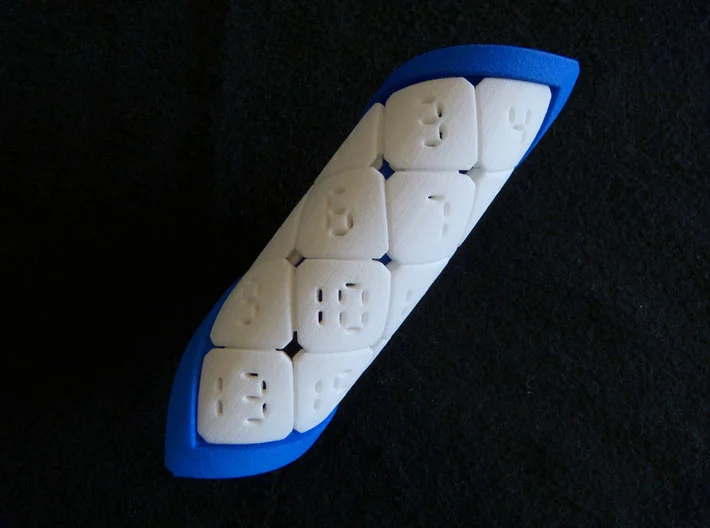
\includegraphics[scale=0.3]{./Figures/coiled15puzzle}
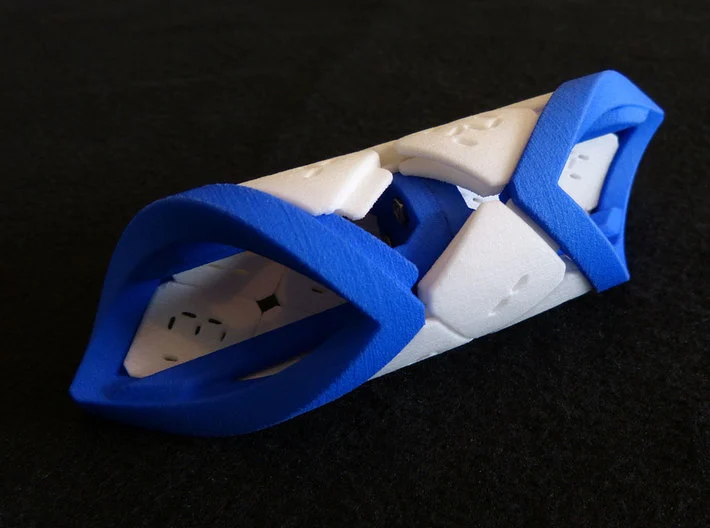
\includegraphics[scale=0.3]{./Figures/coiled15puzzle2.png}
\decoRule
\caption[Coiled 15-puzzle]{Coiled 15-puzzle}
\end{figure}




It is rather easy to see why this is the case, let us discuss why: given a configuration c of the tiles, let us define the permutation p(c) of this configuration according to the following schema: we enumerate the tiles row by row (top to bottom), left to right for odd rows and right to left for the even rows, ignoring the empty compartment. For instance, the following 15-puzzle c:

\begin{fifteen}
\setrow{4}{1,6,2,3}
\setrow{3}{5,10,7,4}
\setrow{2}{9,15,\red14\black,\blue11}
\setrow{1}{13,12,,\blue 8}
\end{fifteen}
\\
\\
we have p(c) = (1, 6, 2, 3, 4, 7, 10, 5, 9, 15, \red 14 \black, \blue 11, 8\black, 12, 13).
\\
It is easy to see that the parity of p(c) cannot change by a legal move of the puzzle. Indeed, p(c) is clearly invariant by lateral move of a tile, so its parity is invariant too. A vertical move of a tile will displace a number in p(c) by an even number of positions right or left. For instance, moving tile 14 into the empty compartment below it results in a new configuration $c_{2}$:

\begin{fifteen}
\setrow{4}{1,6,2,3}
\setrow{3}{5,10,7,4}
\setrow{2}{9,15,,\blue11}
\setrow{1}{13,12,\red14\black,\blue8}
\end{fifteen}
\\
\\
with $p(c_{2})$ = (1, 6, 2, 3, 4, 7, 10, 5, 9, 15, \blue11, 8\black, \red14\black, 12, 13), which is equivalent to moving 14 by 2 positions on the right. This obviously cannot change the parity since exactly 2 pairs of numbers are now in a different order, that is (14, 11) and (14, 8) now appear in the respective opposite orders as (11, 14) and (8, 14).
\\
\\
This is the crux of the proof of the well known necessary condition (even parity of p(c)) for a configuration c to be solvable (see part I of \cite{Johnson1879}).
\\
\\
In the case of the coiled puzzle, we can clearly solve all configurations of even parity, since all the legal moves of the normal puzzle are allowed. In addition, we can for instance transition between the following 2 configurations, which clearly have respectively even and odd parities:

\begin{fifteen}
\centering
\setrow{4}{\red1\black,2,3,4}
\setrow{3}{5,6,7,8}
\setrow{2}{9,10,11,12}
\setrow{1}{13,14,15,}
\end{fifteen}
%
\begin{fifteen}
\setrow{4}{,2,3,4}
\setrow{3}{5,6,7,8}
\setrow{2}{9,10,11,12}
\setrow{1}{13,14,15,\red1\black}
\end{fifteen}
\\
\\
Since it is possible to reach an odd parity configuration, we conclude by invoking symmetry arguments that we can solve all $16!$ configurations. 


%-----------------------------------
%	SUBSECTION 1.2
%-----------------------------------
\subsection{Search Space \& Solvability}

In this thesis, as well as in the code base (\cite{FB}) I have written to do this project, we will consider the general case of a board with n columns and m rows, where $(n, m) \in {\mathbb{N}^{+}}^{2}$, forming $n * m$ compartments. $n * m - 1$ tiles, numbered 1 to $n * m - 1$ are placed in all the compartments but one (which is left empty), and we can slide a tile directly adjascent to the empty compartment into it. Notice from a programming and mathematical analysis perspective, it is often easier to equivalently think of the empty compartment being moved into (or swapped with) an adjacent tile. Starting from a given shuffling of the tiles on the board, our goal will be to execute moves until the are tiles in ascending order: left to right, top to bottom (in the usual western reading order), the empty tile being at the very bottom right.
\\
\\
Note that the case where either n or m is 1 is uninteresting since we can only solve the puzzle if the tiles are in order to start with. For instance, in the (n, 1) case, we can only solve n of the $\frac{n!}{2}$ possible configurations. We will therefore only consider the case where both n and m are strictly greater than 1.
\\
\\
As hinted in the previous section when discussing the coiled 15-puzzle, we can note that the parity argument used there implies that in general, out of the $(n * m)!$ possible permutations of all tiles, only half are attainable and solvable. This gives us a neat way to generate \textit{perfectly shuffled} puzzles, and we make use of this in the code. When comparing various algorithms in later sections, I will compare them on a same set of shuffled puzzles, where the shuffling is either done via a fixed number of random moves from goal position, or via what I call \textit{perfect shuffle}, which means I give equal probability to each attainable configuration of the tiles. A simple way to achieve this is therefore to start with one randomly selected among the $(n * m)!$ permutations, and then to verify that the parity of that permutation is the same as that of the goal (for the given choice of n and m), and simply swap the first two (non-empty) tiles if it is not.




%-----------------------------------
%	SUBSECTION 1.3
%-----------------------------------
\subsection{Optimal Cost \& God's Number}

Let us fix n and m, integers strictly greater than 1 and call $\mathcal{C}_{(n, m)}$ the set of all $\frac{(n * m)!}{2}$ solvable configurations of the n by m sliding-puzzle. For any $c \in \mathcal{C}_{(n, m)}$ we define the optimal cost $\mathcal{O}(c)$ to be the minimum number of moves among all solutions for c. Finally we define $\mathcal{G}(n, m)$, God's number for the n by m puzzle as  $\mathcal{G}(n, m) = \max_{c \in \mathcal{C}_{(n, m)}} \mathcal{O}(c)$. Note that since $\frac{(n * m)!}{2}$ grows rather quickly with n and m, it is impossible to compute $\mathcal{G}$ except in rather trivial cases.
\\
\\
A favourite past time among computer scientists around the glove is therefore to search for more refined lower and upper bounds for $\mathcal{G}(n, m)$, for ever increasing values of n and m. For moderate n and m, we can actually solve optimally all possible configurations of the puzzle and compute exactly $\mathcal{G}(n, m)$  (using for instance $A^{*}$ and an admissible heuristic (recall \ref{GSH}, and we shall see modest examples of that in the results section later). For larger values of n and m (say 5 by 5), we do not know what the God number is. Usually, looking for a lower bound is done by \textit{guessing} hard configurations and computing their optimal path via an optimal search. Looking for upper bounds is done via smart decomposition of the puzzle into disjoint nested regions and for which we can compute an upper bound easily (either by combinatorial analysis or via exhaustive search). See for instance \cite{KarlemoOstergard} for an upper bound of 210 on $\mathcal{G}(5, 5)$.
\\
\\
A very poor lower bound can be always obtained by the following reasoning: each move can at best explore three new configurations (4 possible moves at best if the empty tile is not on a border of the board (less if it is): left, right, up, down but one of which is just going back to an already visited configuration). Therefore, after $p$ moves, we would span at best $\mathcal{S}(p) = \frac{3^{p+1} - 1}{2}$ configurations. A lower bound can thus be obtained for $\mathcal{G}(n, m)$ by computing the smallest integer $p$ for which $\mathcal{S}(p) \ge \frac{(n * m)!}{2}$


%-----------------------------------
%	SECTION 2
%-----------------------------------
\section{Rubik's Cube}



\subsection{History}
The second puzzle I will focus on is the well known Rubik's Cube (\textbf{RC}), invented in 1974 by Erno Rubik, originally known under the name of \textit{Magic Cube} (see \cite{RubiksWiki}). Since it was commericalised in 1980, it has kown a worldwide success: countless people are playing with the famous original 3x3x3 cube, as well as with countless variations, more or less difficult of it. Competitions nowadays bring together \textit{speedcubers} who have trained for years and memorized various algorithms to solve the Rubik's in astonishly effective and fast times (literally in seconds for the best ones). Interestingly, some of the principles used by speedcubers generalise to different dimensions. As an example, it is quite impressive to watch \textit{Cubastic} solve a 15x15x15 RC in two and a half hours (\cite{151515Rubiks}).





\subsection{Search Space \& Solvability}
In my code as well as in this write-up, as is very customary in the RC literature, I will refer to the faces as F (front), B (back), U (up), D (down), L (left) and R (right). The RC's tiles are of 6 different colors, and without loss of generality, we can consider that these colors are also called F, B, U, D, L and R, and consider the goal state as one where, up to rotations of the whole cube, the color's name match the faces (color F on face F, etc). The RC has, as one would expect, an extremely large state space. If we ignore the equivalence via full-cube rotations, there are 24 goal states, since any of the colors can be placed on the F face, and then any of the 4 adjacent colors can be placed on the U face (say). Once these 2 are chosen, the remaining faces are determined. This is not immediately obvious, but not difficult to convince oneself that this is the case with the following two observations about the structure of corner \textit{cubies}: first observation is that they have 3 determined colors, which are fixed once and for all. In particular, the fact that there is no corner with colors F and B, means that once the RC is in solved state, we have to have colors F and B on opposite faces, and similarly for colors U and D as well as colors L and R. Hence, having fixed the color on face F, the color on face B is fixed too. The second observation is that when facing a corner cubie, the order of its three color (e.g. enumerated clock-wise) is invariant. For instance, consider the corner cubie with colors (F, R, U). There is no scrambling of the cube that will produce clock-wise order of e.g. (F, U, R). This is obvious once you consider that there is no move of the Rubik's cube you could not perform while holding a given corner fixed in space (e.g. by pinching that corner cubie with your fingers and never letting go of it).
\\
Finally a further word of notation. It is common in RC jargon to refer to moves  by the name of the face that is rotated clock-wise (when facing it), and by adding a prime \textit{'} for counter-clock-wise rotations. Sometimes people use a number after the face to indicate repeated similar moves, though I will count in my code that as 2 moves, since obviously e.g. U2 = U U = U' U'. As another example: F B' F2 means rotating the front face clock-wise, the back face counter-clock-wise, followed by the front face twice.

\subsubsection{2 x 2 x 2}

Up to rotations of the full RC, there are $\frac{8! * 3^{7}}{24}$ = 3,674,160 possible combinations. Indeed, there are 8! possible ways of choosing the position of the eight corner cubies (since there are known algorithms, such as R’ U R’ D2 R U’ R’ D2 R2, to swap exactly two and only two adjacent corners), each of which can be oriented in 3 different ways (not 6, since as discussed earlier, the clock-wise order of a given corner cubie can never be changed). That gives us $3^8$ permutations of the corners orientation. However, the \textit{corner orientation parity} (\textbf{COP}) (see \cite{Schoenert} for details) is invariant (\% 3) by any legal move of the RC. Since rotating by $120^{o}$ a given corner cubie increases the COP by 1, we conclude that only one third of all these $3^8$ permutations are attainable (namely those for which the COP is equal to 0 \% 3). Finally, the denominator of 24 is due to the equivalence by whole cube rotation as discussed in the previous section.
\\
The insight and knowledge of this section will be useful for me to implement \textit{perfect scrambling} for the 2x2x2 RC. Indeed, the way I generate perfectly shuffled RCs is by randomly placing the 8 corners, then randomly choosing the orientation of the first 7, and finally fixing the $8^{th}$ corner's orientationto make sure COP is equal to 0 \% 3.


\subsubsection{3 x 3 x 3}

TBD

\subsection{Optimal Cost \& God's Number}

\cite{RubiksGodNumber}
\\
\cite{RubiksChicago}
\\
\cite{RubiksRadu}
\\


%-----------------------------------
%	SECTION 3
%-----------------------------------
\section{Solving puzzles \textit{without human knowledge}}

From handcrafted (naive, kociemba) to supervised (DL) to unsupervised (DRL \& DQL) .... but sometimes subtle knowledge injected in e.g. representation or simplifications.



